\label{Schaltungslayout}

In Abbildung \ref{fig:Layout} ist das Schaltungslayout des Projektes zu sehen. Das LCD-Display ist an sechs Pins mit dem Arduino verbunden. Zudem benötigt das LCD eine Versorgungsspannung von ca. 5 Volt. Der Eingang V0 ist dabei über einen Widerstand auf Masse geschalten. Je nach Höhe des Widerstandes ändert sich der Kontrast des LCD-Displays. \\
Darunter befindet sich in der Abbildung \ref{fig:Layout} der CO2-Sensor CCS811, welcher über zwei Pins an den Arduino angeschlossen ist. Einen extra Anschluss an die Versorgungsspannung benötigt dieser nicht, da er die maximal benötigten $3.6$ Volt über den I$^2$C-Anschluss bekommt. \\


\begin{figure}[!hbt]
	\centering
	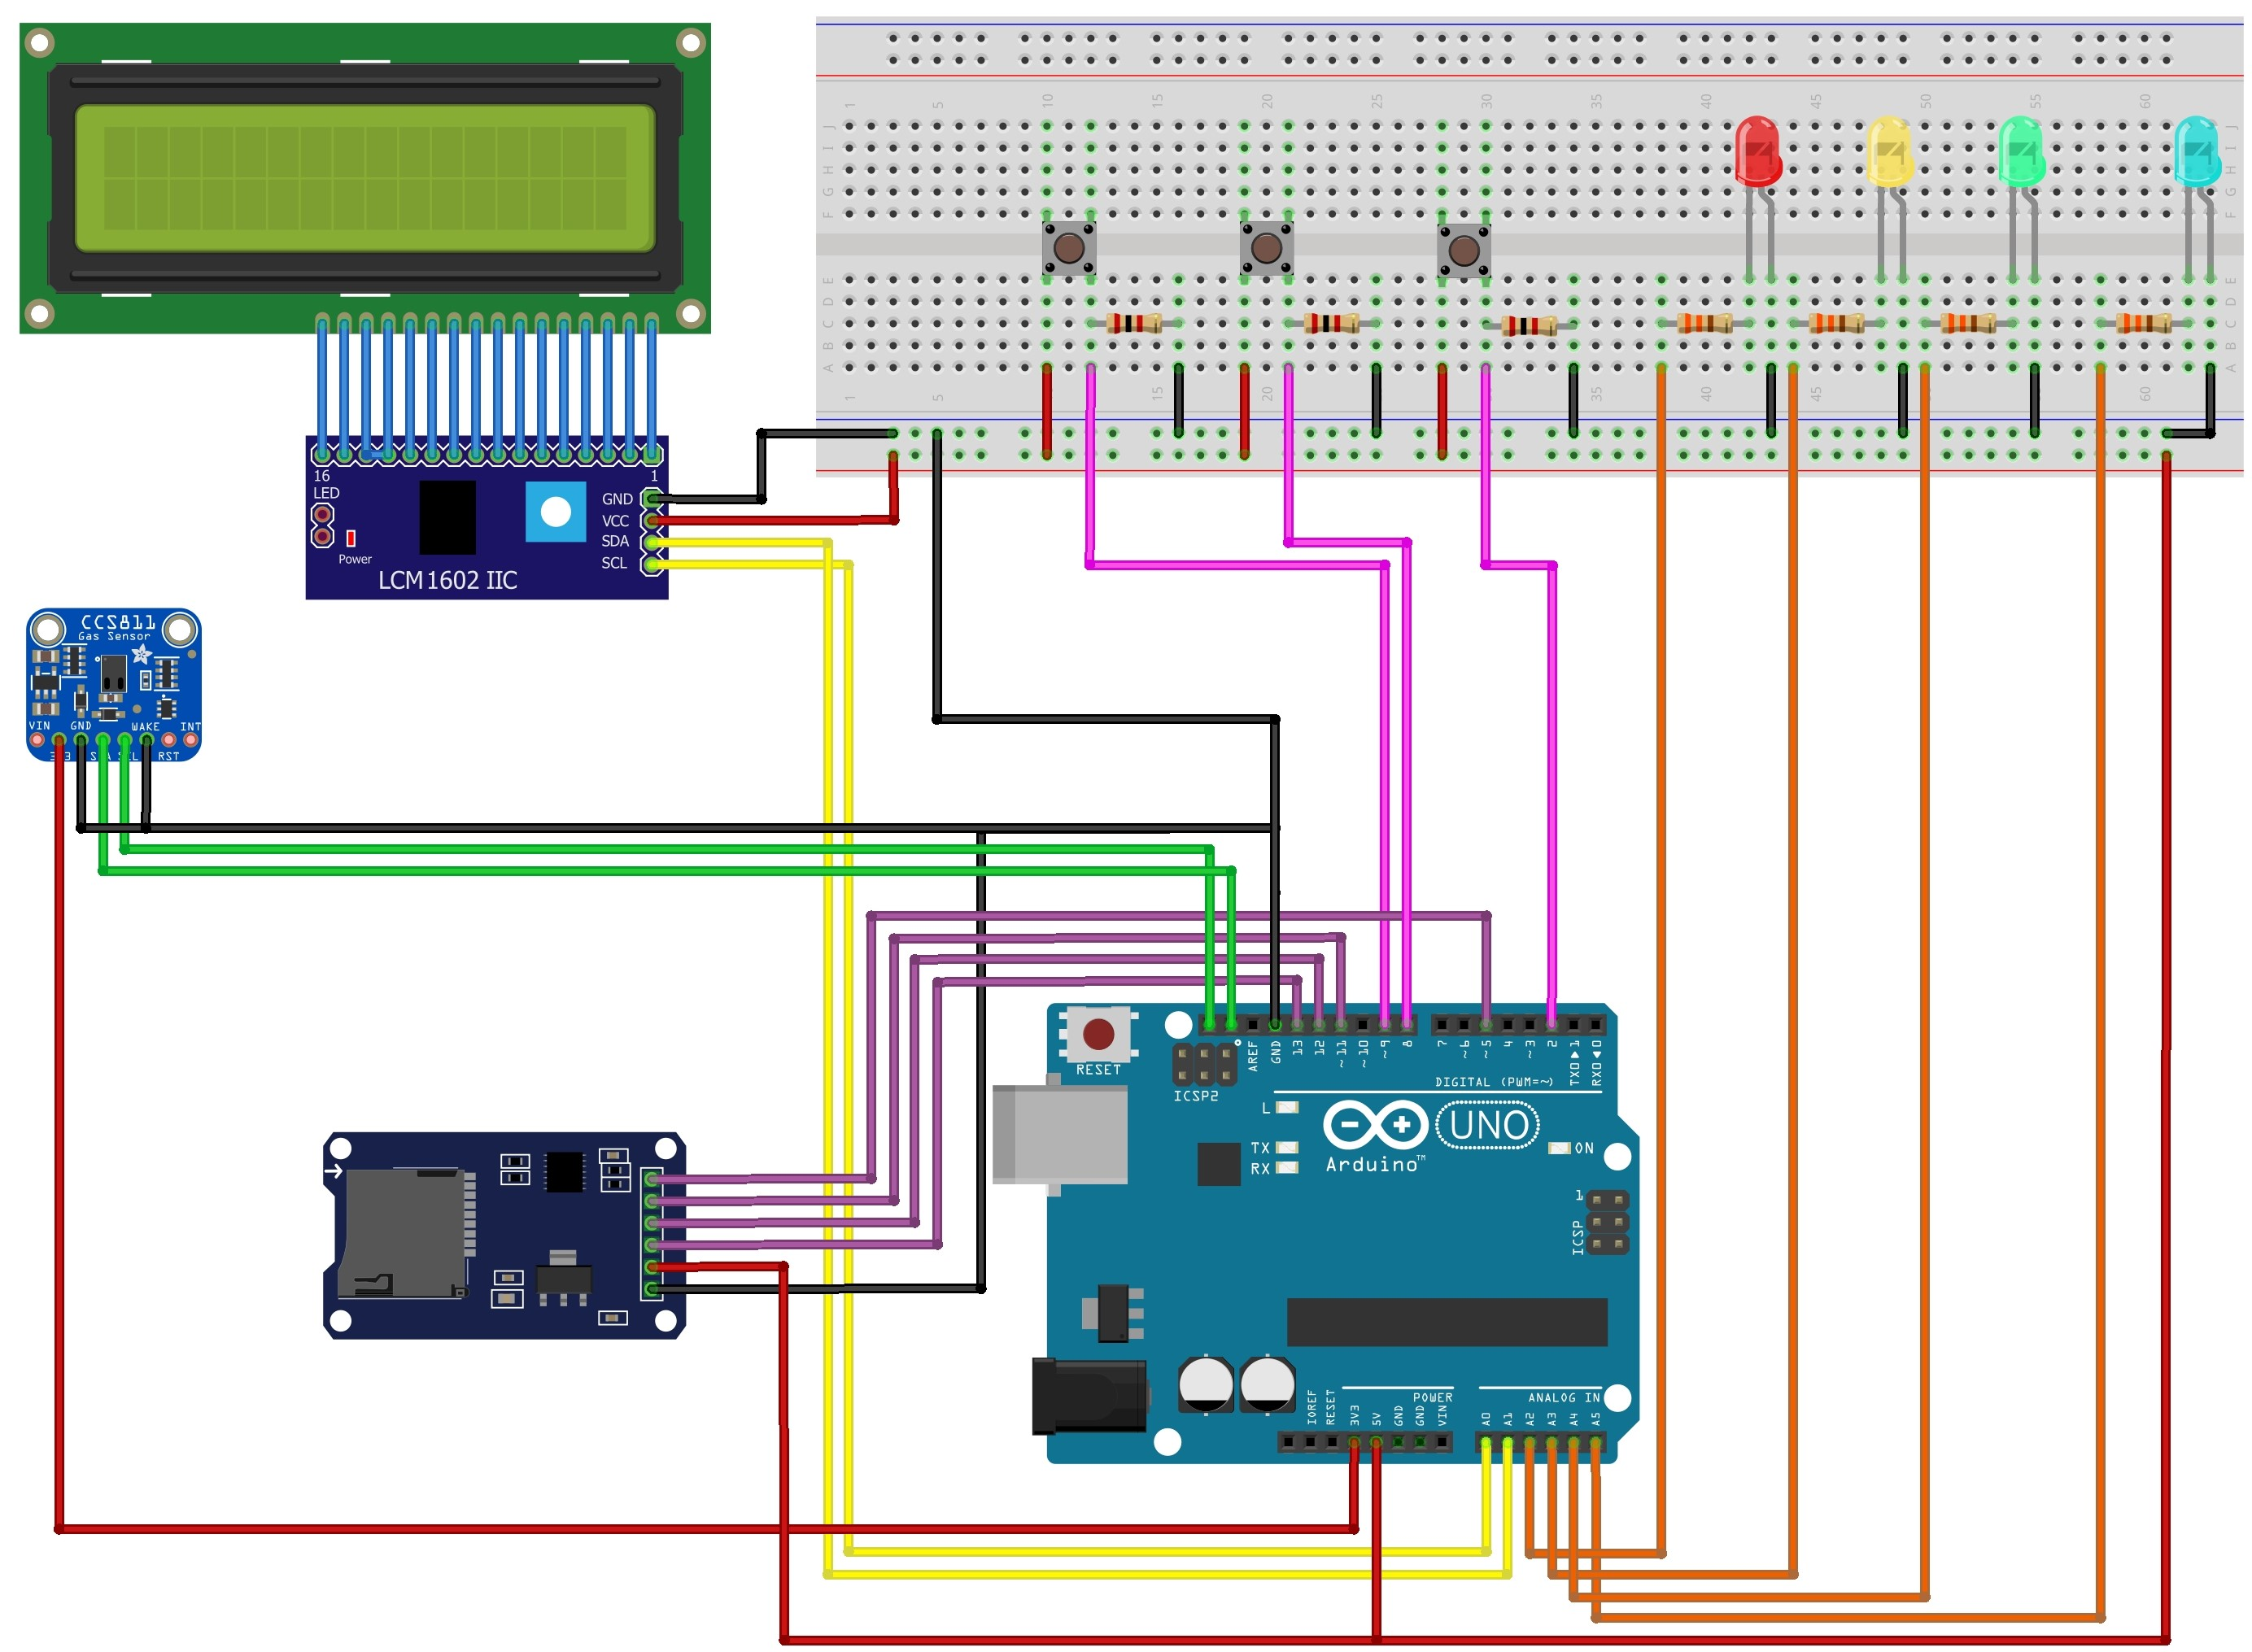
\includegraphics[width=0.9\linewidth]{Images/Layout_Steckplatine}
	\caption{Schaltungslayout vom 27.02.2020}
	\label{fig:Layout}
\end{figure}